\documentclass[10pt,a4paper,titlepage,parskip]{scrartcl}
\usepackage[utf8]{inputenc}
\usepackage{pdfpages}
\usepackage[english]{babel}
\renewcommand\familydefault{\sfdefault}
\usepackage{color}
\usepackage{etoolbox}
\usepackage{lastpage}
\usepackage{hyperref}
\usepackage{framed}
\usepackage{subcaption}

% adjust the page margins
\usepackage[left=2.5cm,right=2.5cm,top=2.5cm,bottom=3.0cm]{geometry}

\usepackage{fancyhdr}
\pagestyle{fancy}

\definecolor{myBlue}{rgb}{0.2,0.4,0.65}
\definecolor{ufzgray1}{RGB}{81,81,81}
\definecolor{ufzgray2}{RGB}{156,156,156}
\definecolor{ufzgray3}{RGB}{185,185,185}

\patchcmd{\headrule}{\hrule}{\color{myBlue}\hrule}{}{}
\patchcmd{\footrule}{\hrule}{\color{myBlue}\hrule}{}{}

% dots after section numbers
\renewcommand{\thesection}{\arabic{section}.}
\renewcommand{\thesubsection}{\arabic{section}.\arabic{subsection}.}

% make an entire region tt font
\newenvironment{ttfont}{\fontfamily{\ttdefault}\selectfont}{\par}

% My style
\usepackage{xcolor}
\definecolor{jmcolor}{RGB}{255,127,0}
\newcommand{\jm}[1]{\textcolor{jmcolor}{#1}}
\newcommand{\jmout}[1]{\textcolor{jmcolor}{\sout{#1}}}
\newcommand{\GRAU}[1]{\textcolor{ufzgray2}{#1}}

%\newcommand{\footrulecolor}{myBlue}
\rhead{}
\chead{\textcolor{myBlue}{\footnotesize Project Documentation ``Improving characterization of flood-producing precipitation events in HFE database''}}
\lfoot{\textcolor{myBlue}{\footnotesize Telephone: +1 (226) 505-5600}}
\cfoot{\textcolor{myBlue}{\footnotesize e-mail: juliane.mai@uwaterloo.ca}}
\rfoot{\textcolor{myBlue}{\footnotesize Page \thepage \ of \pageref{LastPage}}}
\renewcommand{\footrulewidth}{0.4pt} 

% Hurenkinder und Schusterjungen verhindern
\clubpenalty10000
\widowpenalty10000
\displaywidowpenalty=10000

\includepdfset{pages=-}

% colored lines
\makeatletter
\let\old@rule\@rule
\def\@rule[#1]#2#3{\textcolor{rulecolor}{\old@rule[#1]{#2}{#3}}}
\makeatother

% fixed width columns in table
\usepackage{array}
\newcolumntype{L}[1]{>{\raggedright\let\newline\\\arraybackslash\hspace{0pt}}p{#1}}
\newcolumntype{C}[1]{>{\centering\let\newline\\\arraybackslash\hspace{0pt}}p{#1}}
\newcolumntype{R}[1]{>{\raggedleft\let\newline\\\arraybackslash\hspace{0pt}}p{#1}}

%\linespread{1.5}

\begin{document}  
	
	\vspace*{-1cm}
	\pagestyle{fancy}
	
	\begin{center}
		Juliane Mai, Ph.D.\\
		Technical Consulting\\[4pt]
		405-460A Belmont Ave W., \\
		Kitchener, ON, N2M 0A9, Canada\\[10pt]
		{\definecolor{rulecolor}{named}{myBlue}\rule{\linewidth}{0.4pt}}
	\end{center}
	\begin{center}
		\textcolor{myBlue}{{\Large --~Documentation~--}}\\[4pt]
		Improving the characterization of the flood-producing precipitation events in the Historic Flood Event (HFE) database by using the CaPA reanalysis/analysis\\[4pt]
	\end{center}
	

\vspace*{0cm}

\section{Meetings}

\subsection{Kick-off Meeting}
\vspace*{-0.5cm}
\begin{tabbing}
	\hspace{2.8cm} \= \hspace{4cm} \= \kill \\
	\textbf{Date and time:} 	\> Aug 25, 2022 1-2pm\\
	\textbf{Attendees:} 	\> Dikra Khedhaouiria \> (dikraa.khedhaouiria@ec.gc.ca)\\
							\> Juliane Mai \> (juliane.mai@uwaterloo.ca)\\
							\> Marie-Eve Martin \> (marie-eve.martin@nrcan-rncan.gc.ca)\\
							\> Philippe Aussant \> (philippe.aussant@NRCan-RNCan.gc.ca)\\
	                        \> Pierre-Etienne Bonhomme \> (etienne.bonhomme@NRCan-RNCan.gc.ca)\\
	                        \> Vincent Fortin \> (vincent.fortin@ec.gc.ca)
\end{tabbing}
\vspace*{-0.5cm}
\textbf{Notes:}
\begin{itemize}
	\setlength\itemsep{-0.8em}
	\item discussion of access to resources (HFE database, Geomet requests, CaSPAr requests)
	\item discussion of formats (JSON, PNG, i.e., mimicking formats that are received when requesting data from GeoMet)
	\item discussion of handling liquid/solid precipitation (Vincent suggested manuscript in preparation that will require humidity and temperature as additional variables to transform precipitation into components)
	\item next meeting mid September will be scheduled by Dikra
\end{itemize}

\section{Resources}

\begin{itemize}
	\setlength\itemsep{-0.8em}
	\item access to the HFE database:\\
	\url{https://open.canada.ca/data/en/dataset/fe83a604-aa5a-4e46-903c-685f8b0cc33c}
	\item query to obtain RDPA 24h total precipitation for a 1x1 degree box centered on Montreal:\\
	\url{https://api.weather.gc.ca/collections/weather:rdpa:10km:24f/coverage?f=json&datetime=2017-05-12T12Z&CRS=EPSG:4326&bbox=-74,45,-73,46}
	\item documentation of requests from GeoMet:\\
	\url{https://eccc-msc.github.io/open-data/msc-geomet/web-services_en/}\\
	see specifically OGC API:\\
	\url{https://eccc-msc.github.io/open-data/msc-geomet/web-services_en/#ogc-api-features}
\end{itemize}
\pagebreak

\section{Request, read, and plot data from GeoMet}

The assumption is that we want to retrieve CaPA data (RDPA; 24h total precipitation) from GeoMet for Aug 9, 2018 around Montreal ($\mathrm{lat} = 45.5019^{\circ}\mathrm{N}$, $\mathrm{lon}=-73.5674^{\circ}\mathrm{E}$). 

The URL to request is the following:
\url{https://api.weather.gc.ca/collections/weather:rdpa:10km:24f/coverage?f=json&datetime=2022-08-24T12Z&CRS=EPSG:4326&bbox=-74,45,-73,46}

This returns the following JSON string (not geo-referenced):
\begin{framed}	
		\texttt{\{"type": "Coverage", "domain": \{"type": "Domain", "domainType": "Grid", "axes": \{"x": \{"start": -74.0, "stop": -73.0, "num": 15\}, "y": \{"start": 46.0, "stop": 45.0, "num": 16\}\}, "referencing": [\{"coordinates": ["x", "y"], "system": \{"type": "GeographicCRS", "id": "http://www.opengis.net/def/crs/OGC/1.3/CRS84"\}\}]\}, "parameters": \{"APCP": \{"type": "Parameter", "description": "Total precipitation [kg/(m\^{}2)]", "unit": \{"symbol": "[kg/(m\^{}2)]"\}, "observedProperty": \{"id": "0-SFC", "label": \{"en": "Total precipitation [kg/(m\^{}2)]"\}\}\}\}, "ranges": \{"APCP": \{"type": "NdArray", "dataType": "float", "axisNames": ["y", "x"], "shape": [16, 15], "values": [null, null, null, null, null, null, null, null, null, null, null, null, null, null, null, null, null, null, null, null, null, 9.300250053405762, 12.344250679016113, null, null, null, null, null, null, null, null, null, null, null, null, 5.607500076293945, 9.330750465393066, 13.382000923156738, 16.639751434326172, null, null, null, null, null, null, $\ldots$ , null, null, null, null, null, null, null, 10.574250221252441, 11.665250778198242, 11.032000541687012, null, null, null, null, null, null, null, null, null, null, null, null, 9.582500457763672, 10.17750072479248, null, null, null, null, null, null, null, null, null, null, null, null, null, null, null, null, null, null, null, null, null]\}\}\}}\\
\end{framed}

This corresponds to the following 2D view of the data (not geo-referenced):
\begin{table}[h]
	\begin{tabular}{R{0.5cm}R{0.5cm}R{0.5cm}R{0.5cm}R{0.5cm}R{0.5cm}R{0.5cm}R{0.5cm}R{0.5cm}R{0.5cm}R{0.5cm}R{0.5cm}R{0.5cm}R{0.5cm}R{0.5cm}}
- & - & - & - & - & - & - & - & - & - & - & - & - & - & -\\
- & - & - & - & - & - & 9 & 12 & - & - & - & - & - & - & -\\
- & - & - & - & - & 6 & 9 & 13 & 17 & - & - & - & - & - & -\\
- & - & - & - & 4 & 6 & 9 & 13 & 17 & 21 & - & - & - & - & -\\
- & - & 3 & 3 & 4 & 6 & 11 & 16 & 19 & 22 & - & - & - & - & -\\
- & 4 & 3 & 3 & 3 & 6 & 13 & 18 & 22 & 25 & 23 & - & - & - & -\\
- & 5 & 4 & 3 & 3 & 5 & 12 & 19 & 23 & 28 & 26 & 28 & - & - & -\\
- & - & 5 & 3 & 2 & 4 & 12 & 18 & 23 & 26 & 27 & 32 & 38 & - & -\\
- & - & - & 3 & 2 & 4 & 10 & 16 & 20 & 22 & 26 & 35 & 38 & 27 & -\\
- & - & - & - & 4 & 5 & 8 & 16 & 18 & 20 & 27 & 36 & 35 & 24 & -\\
- & - & - & - & 6 & 6 & 7 & 14 & 16 & 20 & 31 & 41 & 35 & 20 & -\\
- & - & - & - & - & 5 & 8 & 11 & 13 & 16 & 27 & 37 & 33 & - & -\\
- & - & - & - & - & - & 10 & 10 & 12 & 11 & 19 & 26 & - & - & -\\
- & - & - & - & - & - & - & 11 & 12 & 11 & - & - & - & - & -\\
- & - & - & - & - & - & - & 10 & 10 & - & - & - & - & - & -\\
- & - & - & - & - & - & - & - & - & - & - & - & - & - & -\\				
	\end{tabular}
\end{table}
\pagebreak

To retrieve the corresponding PNG file for this data use (see Fig.~\ref{fig:plot_example:geo-weather}) (not geo-referenced):
\begin{framed}
\url{https://geo.weather.gc.ca/geomet?SERVICE=WMS&VERSION=1.3.0&REQUEST=GetMap&LAYERS=RDPA.24F_PR&STYLES=RDPA-WXO&CRS=EPSG:4326&BBOX=45,-74,46,-73&WIDTH=400&HEIGHT=400&FORMAT=image/png&TIME=2022-08-24T12:00:00Z&DIM_REFERENCE_TIME=2022-08-24T12:00:00Z}
\end{framed}
To retrieve the legend use (see Fig.~\ref{fig:plot_example:geo-weather}):
\begin{framed}
	\url{https://geo.weather.gc.ca/geomet?SERVICE=WMS&VERSION=1.3.0&REQUEST=GetLegendGraphic&LAYERS=RDPA.24F_PR&STYLES=RDPA-WXO&CRS=EPSG:4326&BBOX=45,-74,46,-73&WIDTH=400&HEIGHT=400&FORMAT=image/png&TIME=2022-08-24T12:00:00Z&DIM_REFERENCE_TIME=2022-08-24T12:00:00Z}
\end{framed}

To actually retrieve the geo-referenced data used for those plots, the GRIB2 file needs to be retrieved using the following command:
\begin{framed}
\texttt{\url{https://api.weather.gc.ca/collections/weather:rdpa:10km:24f/coverage?f=GRIB&datetime=2022-08-24T12Z&CRS=EPSG:4326&bbox=-74,45,-73,46}}
\end{framed}
This seems to be the only possibility to obtain geo-referenced data. The library developed here now provides three functions to obtain and plot the data. The results are shown in Fig.~\ref{fig:plot_example:api-weather}.

\textbf{Step A1:} Request data using the Geomet API (\url{https://api.weather.gc.ca}).
\begin{framed}
	\vspace*{-1.2cm}
	\begin{ttfont}
	\begin{tabbing}
		\hspace{1.0cm} \= \hspace{3.2cm} \= \kill \\[4pt]
		\GRAU{\# see module for detailed documentation and example}\\
		from a1\_request\_geomet\_grib2 import request\_geomet\_grib2\\
		\\
		files\_geomet = request\_geomet\_grib2(\\
		\> \GRAU{\# Mandatory arguments:}\\
		\> product=\textit{product}, \> \GRAU{\# name of product, e.g., ``rdpa:10km:24f''}\\
		\> date=\textit{date},\> \GRAU{\# datetime object specifying date (can be list of dates)}\\
		\> bbox=\textit{bbox},\> \GRAU{\# dictionary specifying bounding box}\\
		\> \GRAU{\# Optional arguments:}\\
		\> crs=\textit{crs},\> \GRAU{\# coordinate reference system, e.g., ``EPSG:4326''}\\
		\> filename=\textit{filename},\> \GRAU{\# base filename of output file (can include path but no}\\
		\>                           \> \GRAU{\# file extension); date will be added to filename}\\
		\> silent=\textit{silent}, \> \GRAU{\# True for no printing on screen}\\
		\> ) \> 
	\end{tabbing}
	\end{ttfont}
	\vspace*{-0.3cm}
\end{framed}
\vspace*{-0.3cm}
The return variable \texttt{files\_geomet} is a list of files requested and downloaded. If the file already existed, it will not be overwritten unless \texttt{overwrite} is set to \texttt{True}. The filename will be returned nonetheless. 

\textbf{Step B1:} Read data from files requested.
\begin{framed}
	\vspace*{-1.2cm}
	\begin{ttfont}
		\begin{tabbing}
			\hspace{1.0cm} \= \hspace{5.2cm} \= \kill \\[4pt]
			\GRAU{\# see module for detailed documentation and example}\\
			from b1\_read\_geomet\_grib2 import read\_geomet\_grib2\\
			\\
			data\_geomet = read\_geomet\_grib2(\\
			\> \GRAU{\# Mandatory arguments:}\\
			\> filenames=\textit{files\_geomet}, \> \GRAU{\# list of GRIB2 files to read}\\
			\> \GRAU{\# Optional arguments:}\\
			\> lintransform=\textit{lintransform}, \> \GRAU{\# dictionary to specify linear transform of}\\
			\>  \> \GRAU{\# data, e.g., to allow for unit conversions}\\
			\> silent=\textit{silent}, \> \GRAU{\# True for no printing on screen}\\
			\> ) \> 
		\end{tabbing}
	\end{ttfont}
	\vspace*{-0.3cm}
\end{framed}
\vspace*{-0.3cm}
The returned variable \texttt{data\_geomet} is a dictionary that will contain the attributes \texttt{lat}, \texttt{lon}, and \texttt{var}. The latter will be 3-dimensional if several files were read. The latitude and longitudes of the files are checked for consistency.

\textbf{Step Cx:} Plot data.
\begin{framed}
	\vspace*{-1.2cm}
	\begin{ttfont}
		\begin{tabbing}
			\hspace{1.0cm} \= \hspace{5.2cm} \= \kill \\[4pt]
			\GRAU{\# see module for detailed documentation and example}\\
			from cx\_plot\_data import plot\_data\\
			\\
			plot\_geomet = plot\_data(\\
			\> \GRAU{\# Mandatory arguments:}\\
			\> var=\textit{var}, \> \GRAU{\# 2D/3D array of values for variable}\\
			\> lat=\textit{lat}, \> \GRAU{\# 2D array of latitudes}\\
			\> lon=\textit{lon}, \> \GRAU{\# 2D array of longitudes}\\
			\> date=\textit{date}, \> \GRAU{\# date or list of dates as datetime objects}\\
			\> \GRAU{\# Optional arguments:}\\
			\> png=\textit{png}, \> \GRAU{\# True if PNG file(s) should be created}\\
			\> gif=\textit{gif}, \> \GRAU{\# True if GIF should be created}\\
			\> legend=\textit{legend}, \> \GRAU{\# True if PNG of legend should be created}\\
			\> cities=\textit{cities}, \> \GRAU{\# True to display cities on maps}\\
			\> bbox=\textit{bbox}, \> \GRAU{\# Bounding box will be plotted if provided}\\
			\> basefilename=\textit{basefilename}, \> \GRAU{\# String specifying basename of files created}\\
			\> silent=\textit{silent}, \> \GRAU{\# True for no printing on screen}\\
			\> ) \> 
		\end{tabbing}
	\end{ttfont}
	\vspace*{-0.3cm}
\end{framed}
\vspace*{-0.3cm}
The returned variable \texttt{plot\_geomet} is a dictionary that will contain the attributes \texttt{png}, \texttt{gif}, and \texttt{legend}. Each of them are assigned list of the according files created. If no file was created (e.g., no legend), the respective list will be empty.

\begin{figure}[h]
	\begin{subfigure}[b]{0.45\textwidth}
		\centering
		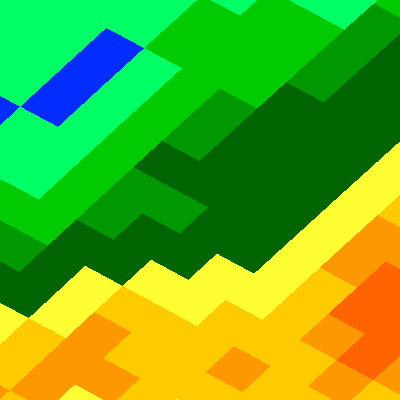
\includegraphics[height=0.58\linewidth]{figures/test-map-geomet-geo-weather-rdpa24_2018080912.png}
		\hspace*{0.5cm}
		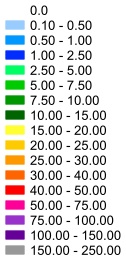
\includegraphics[height=0.58\linewidth]{figures/test-map-geomet-geo-weather-rdpa24_legend.png}
		\caption{Raw PNG and legend for RDPA-24h data retrieved using \url{https://geo.weather.gc.ca}\\(only displayed for reference)}
		\label{fig:plot_example:geo-weather}
	\end{subfigure}
	\hspace*{0.05\textwidth}
	\begin{subfigure}[b]{0.45\textwidth}
		\centering
		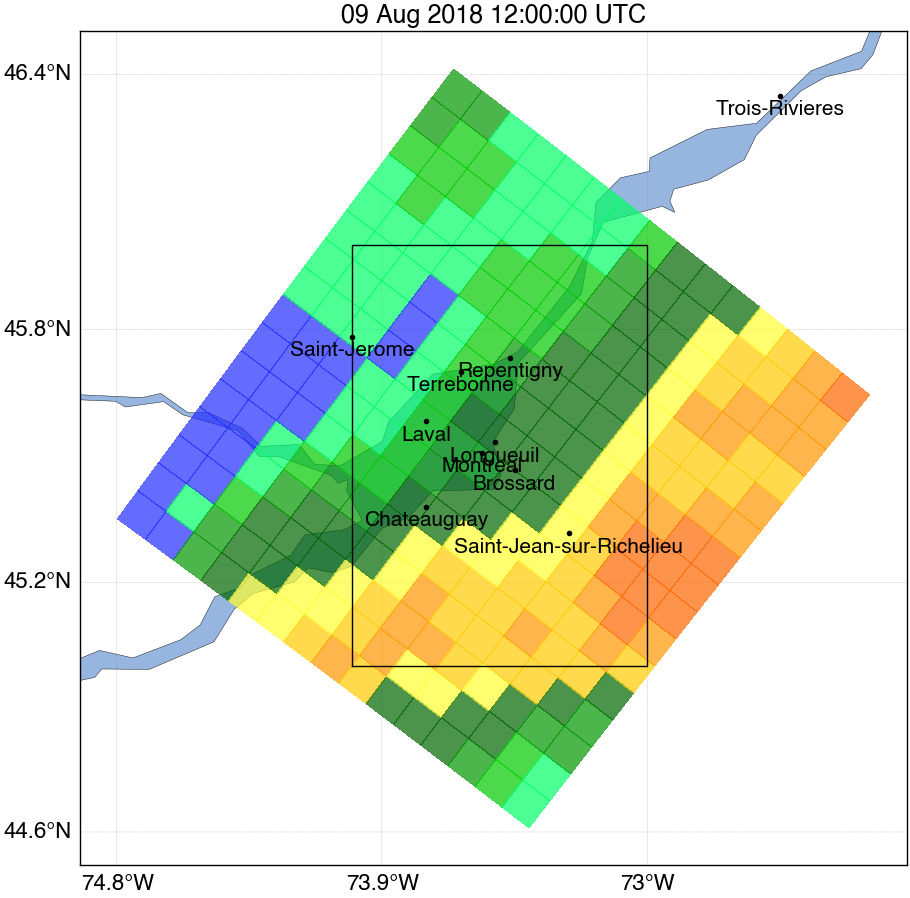
\includegraphics[height=0.58\linewidth]{figures/test-map-geomet-nrcan-hfe-rdpa24_2018080912.png}
		\hspace*{0.5cm}
		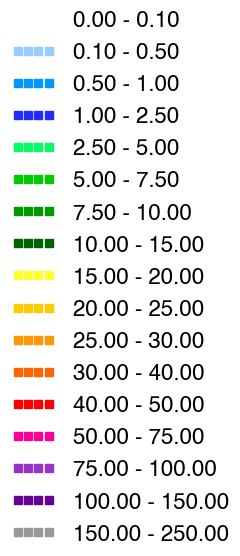
\includegraphics[height=0.58\linewidth]{figures/test-map-geomet-nrcan-hfe-rdpa24_legend.png}
		\caption{PNG and legend produced using NRCan-HFE library based on GRIB2 data (RDPA-24h) retrieved using \url{https://api.weather.gc.ca/}}
		\label{fig:plot_example:api-weather}
	\end{subfigure}
	\caption{RDPA (24h total precipitation) on Aug 9, 2018 (noon UTC) around Montreal}
	\label{fig:plot_example_geomet-api_vs_geomet-nrcan-hfe}
\end{figure}

\pagebreak

\section{Request, read, and plot data from CaSPAr}

\textbf{Step A2:} Request data using CaSPAr (\url{https://caspar-data.ca/caspar}).

The following function is just a dummy to provide some information on how to retrieve data from CaSPAr manually. Fig.~\ref{fig:request_data_caspar} shows the setting used to retrieve RDRS-v2.1 data from CaSPAr. The shapefile containing the domain of the HFE database is provided under \texttt{data/caspar/RDRS\_v21\_hfe\_outline.zip}. Some example data are made available (see \texttt{src/test-data/*.nc}). See more information on how to create a CaSPar account, request and dwonload data under \url{https://github.com/julemai/CaSPAr/wiki/How-to-get-started-and-download-your-first-data}.
\begin{framed}
	\vspace*{-1.2cm}
	\begin{ttfont}
		\begin{tabbing}
			\hspace{1.0cm} \= \hspace{3.2cm} \= \kill \\[4pt]
			\GRAU{\# see module for detailed documentation and example}\\
			from a2\_request\_caspar\_nc import request\_caspar\_nc\\
			\\
			files\_caspar = request\_caspar\_nc( ) \> 
		\end{tabbing}
	\end{ttfont}
	\vspace*{-0.3cm}
\end{framed}
\vspace*{-0.3cm}
The return variable \texttt{files\_caspar} is 0. The function will only display a warning that the data have to be requested and downloaded manually. 
\begin{figure}[h]
	\centering
	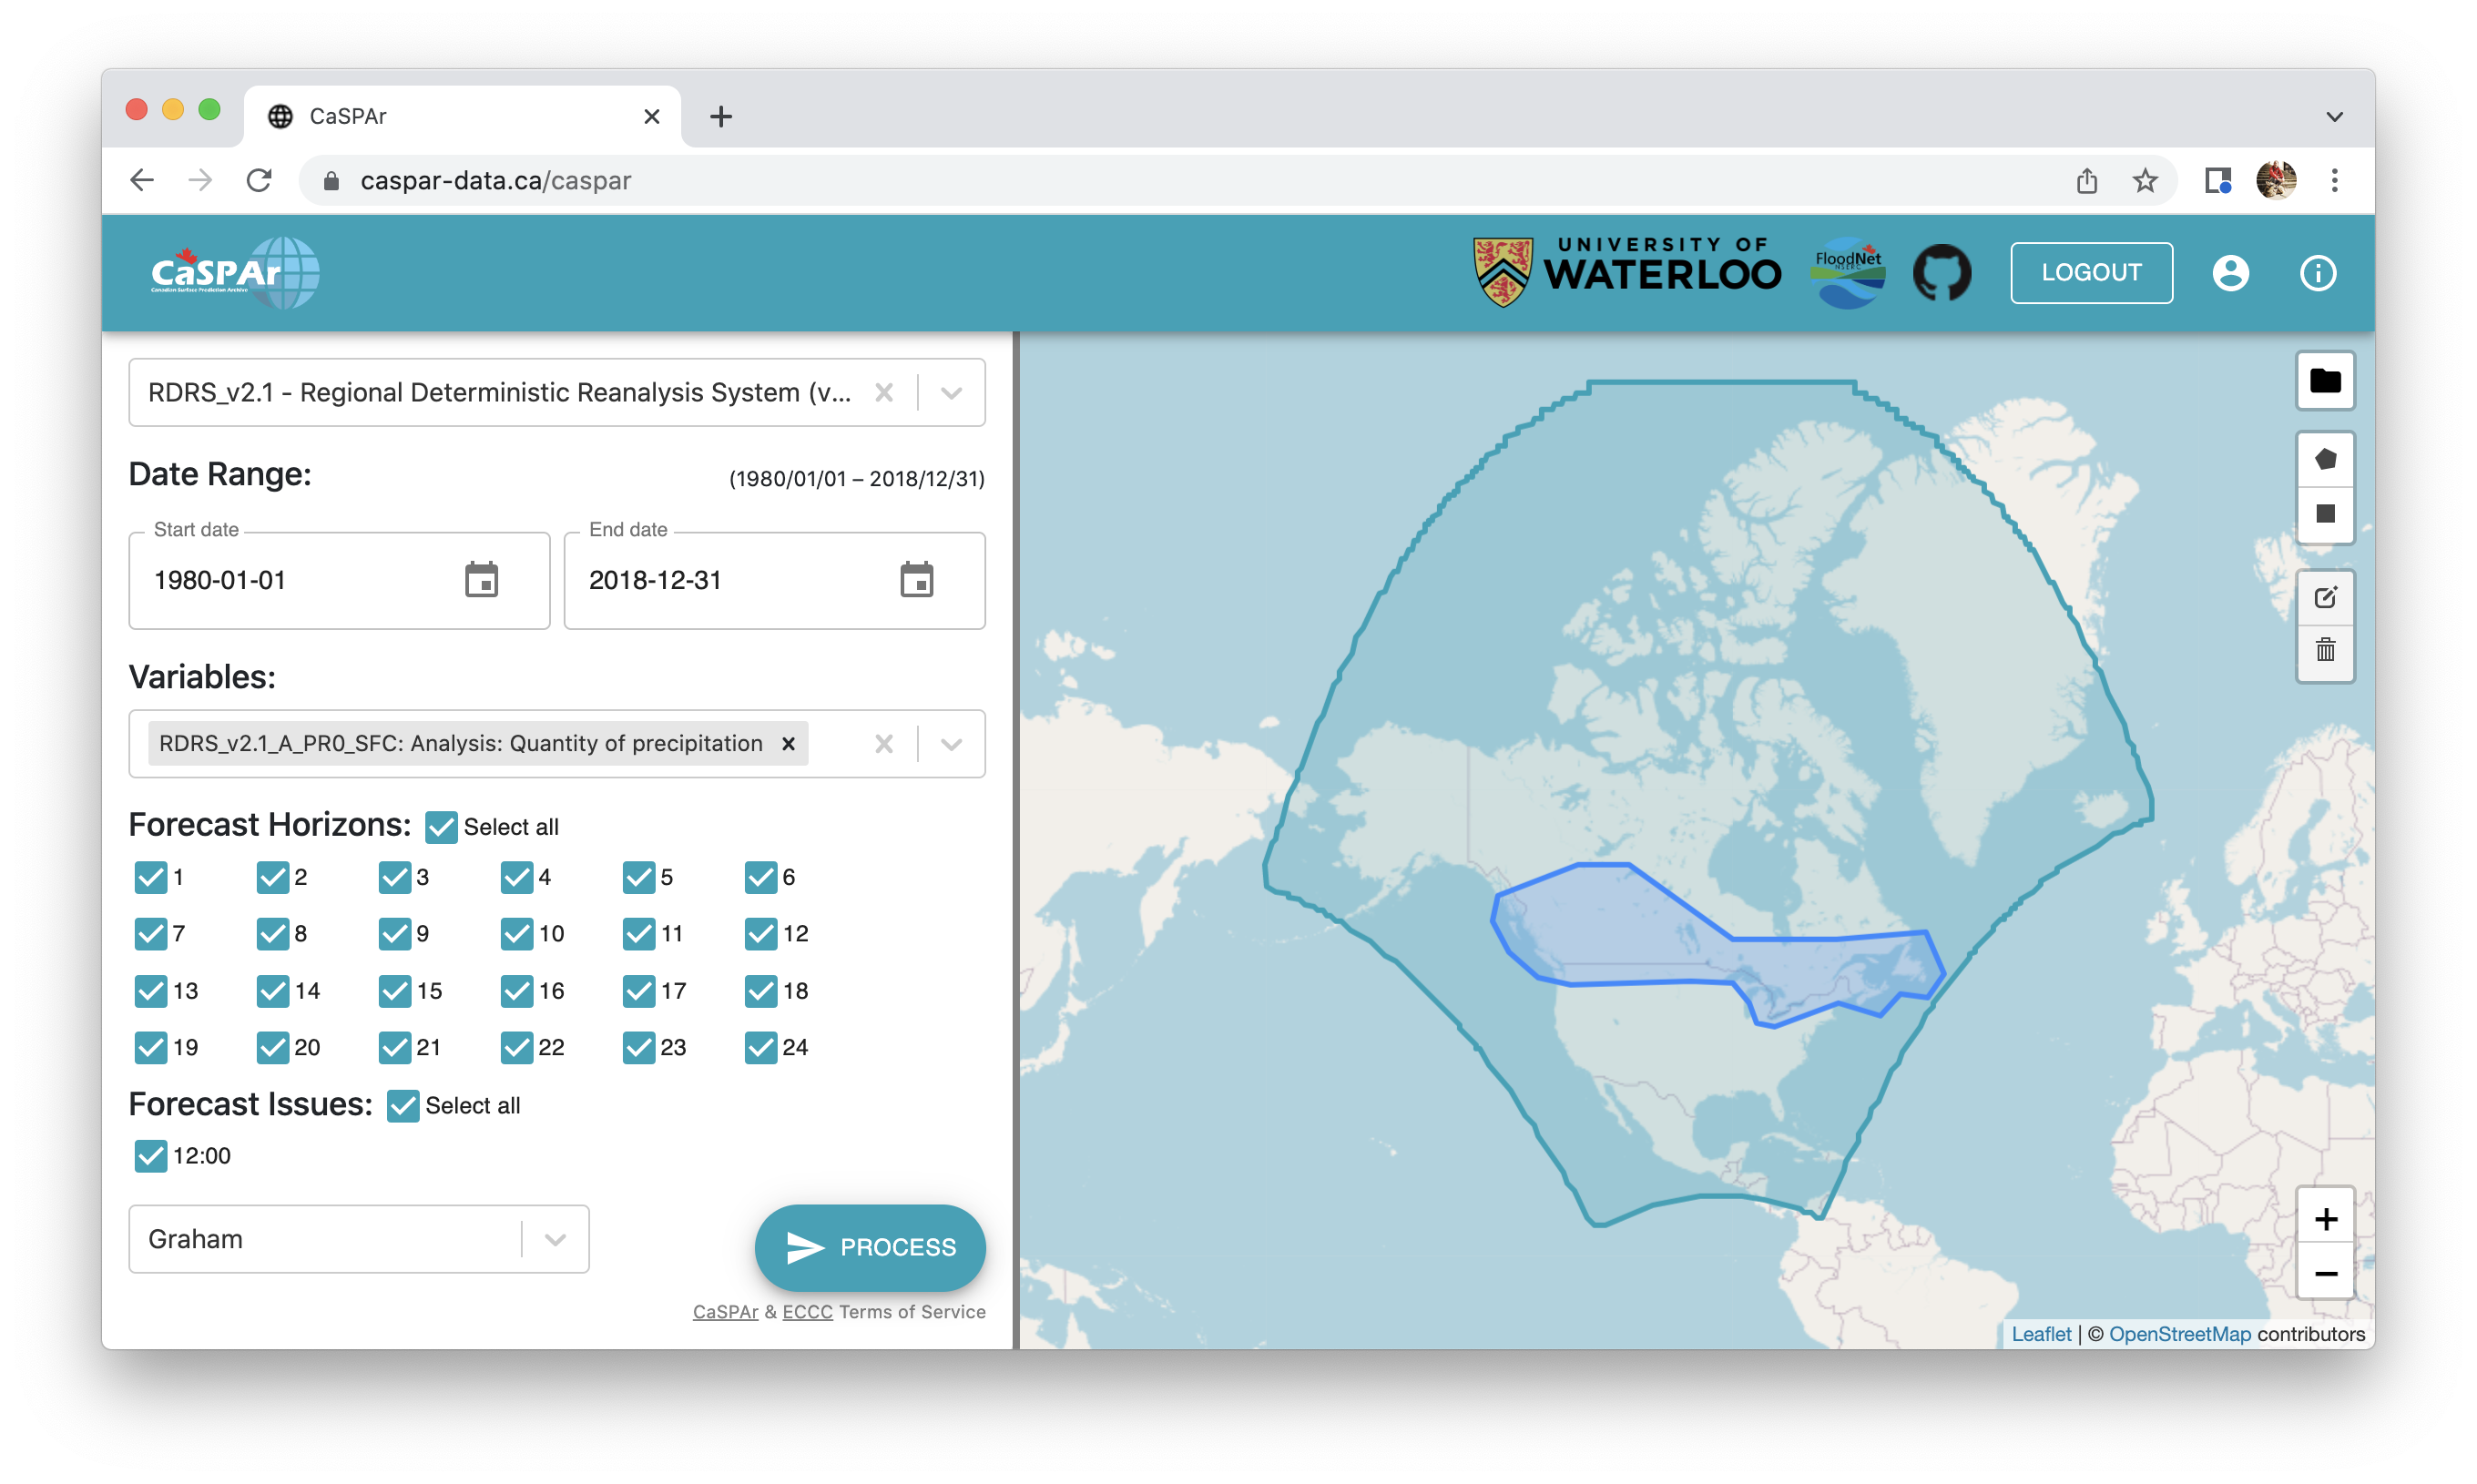
\includegraphics[width=\linewidth]{figures/caspar-request-hfe.png}
	\caption{Screenshot of CaSPAr (\url{https://caspar-data.ca/caspar}) frontend displaying setting to request RDRS-v2.1 for the HFE domain. The shapefile used to define the domain (blue highlighted area) within the data available for RDRS-v2.1 (turquoises highlighted area) is available under \texttt{data/caspar/RDRS\_v21\_hfe\_outline.zip} and has been used via file upload (top button in right top corner of the map).}
	\label{fig:request_data_caspar}
\end{figure}

\textbf{Step B2:} Read data from CaSPAr files.
\begin{framed}
	\vspace*{-1.2cm}
	\begin{ttfont}
		\begin{tabbing}
			\hspace{1.0cm} \= \hspace{5.2cm} \= \kill \\[4pt]
			\GRAU{\# see module for detailed documentation and example}\\
			from b2\_read\_caspar\_nc import read\_caspar\_nc\\
			\\
			data\_caspar = read\_caspar\_nc(\\
			\> \GRAU{\# Mandatory arguments:}\\
			\> product=\textit{product}, \> \GRAU{\# name of product in CaSPAr (e.g., 'RDRS-v2.1')}\\
			\> variable=\textit{variable}, \> \GRAU{\# name of variable in CaSPAr}\\
			\> \> \GRAU{\#  (e.g., 'RDRS\_v2.1\_A\_PR0\_SFC')}\\
			\> date=\textit{date}, \> \GRAU{\# datetime object specifying date}\\
			\> \> \GRAU{\#  (can be list of dates)}\\
			\> \GRAU{\# Optional arguments:}\\
			\> bbox=\textit{bbox}, \> \GRAU{\# dictionary specifying bounding box}\\
			\> foldername=\textit{foldername}, \> \GRAU{\# name of folder that contains files requested}\\
			\> \> \GRAU{\# and downloaded from CaSPAr (files not renamed)}\\
			\> lintransform=\textit{lintransform}, \> \GRAU{\# dictionary to specify linear transform of}\\
			\>  \> \GRAU{\# data, e.g., to allow for unit conversions}\\
			\> silent=\textit{silent}, \> \GRAU{\# True for no printing on screen}\\
			\> ) \> 
		\end{tabbing}
	\end{ttfont}
	\vspace*{-0.3cm}
\end{framed}
\vspace*{-0.3cm}
The returned variable \texttt{data\_caspar} is a dictionary that will contain the attributes \texttt{lat}, \texttt{lon}, and \texttt{var}. The latter will be 3-dimensional if several dates were read. The latitude and longitudes of the files are checked for consistency.

\textbf{Step Cx:} Plot data.

Since the data \texttt{data\_caspar} have the same structure as the data read from Geomet (i.e., \texttt{data\_geomet}) the plotting of the data is now exactly the same. See \textbf{Step Cx} above. 

\begin{framed}
	\vspace*{-1.2cm}
	\begin{ttfont}
		\begin{tabbing}
			\hspace{1.0cm} \= \hspace{5.2cm} \= \kill \\[4pt]
			\GRAU{\# see module for detailed documentation and example}\\
			from cx\_plot\_data import plot\_data\\
			\\
			plot\_caspar = plot\_data(\\
			\> \GRAU{\# Mandatory arguments:}\\
			\> var=data\_caspar["var"], \> \GRAU{\# 2D/3D array of values for variable}\\
			\> lat=data\_caspar["lat"], \> \GRAU{\# 2D array of latitudes}\\
			\> lon=data\_caspar["lon"], \> \GRAU{\# 2D array of longitudes}\\
			\> ... \> \GRAU{\# see above "Step Cx" for more arguments }\\
			\> ) \> 
		\end{tabbing}
	\end{ttfont}
	\vspace*{-0.3cm}
\end{framed}
\vspace*{-0.3cm}
The returned variable \texttt{plot\_caspar} is a dictionary that will contain the attributes \texttt{png}, \texttt{gif}, and \texttt{legend}. Each of them are assigned list of the according files created. If no file was created (e.g., no legend), the respective list will be empty.

Fig.~\ref{fig:plot_example:caspar} shows the result of a plot of precipitation (\texttt{RDRS-v2.1\_A\_PR0\_SFC}) in the RDRS-v2.1 product for a domain around Montreal on Aug 9, 2018 at 7:00 am (UTC). For comparison, the other two panels in this figure (i.e., Fig.~\ref{fig:plot_example:api-weather:24h} and Fig.~\ref{fig:plot_example:api-weather:6h}) show the results of plotting data requested from Geomet for the same day but as 24-h and 6-h precipitation accumulations of the RDPA product.

\begin{figure}[h]
	\begin{subfigure}[a]{0.27\textwidth}
		\centering
		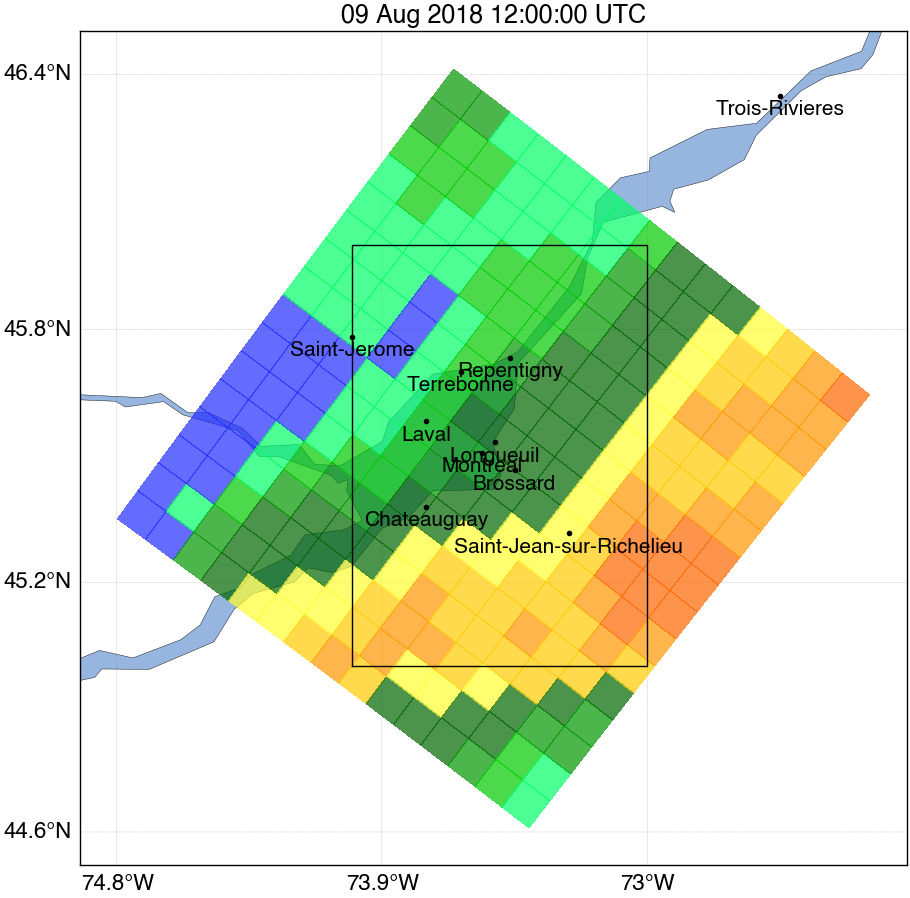
\includegraphics[height=0.9\linewidth]{figures/test-map-geomet-nrcan-hfe-rdpa24_2018080912.png}
		\caption{PNG produced using NRCan-HFE library based on GRIB2 data (RDPA-24h) retrieved using \url{https://api.weather.gc.ca/}}
		\label{fig:plot_example:api-weather:24h}
	\end{subfigure}
	\hspace*{0.02\textwidth}
	\begin{subfigure}[a]{0.27\textwidth}
		\centering
		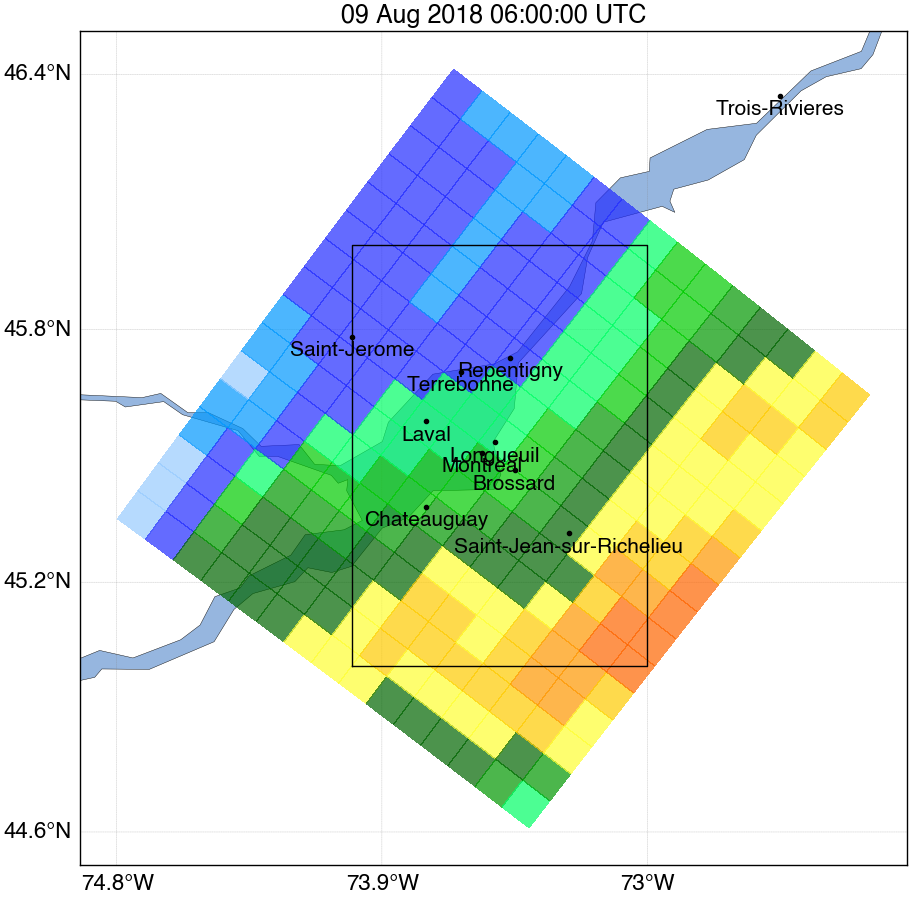
\includegraphics[height=0.9\linewidth]{figures/test-map-geomet-nrcan-hfe-rdpa6_2018080906.png}
		\caption{PNG produced using NRCan-HFE library based on GRIB2 data (RDPA-6h) retrieved using \url{https://api.weather.gc.ca/}}
		\label{fig:plot_example:api-weather:6h}
	\end{subfigure}
	\hspace*{0.02\textwidth}
	\begin{subfigure}[a]{0.27\textwidth}
		\centering
		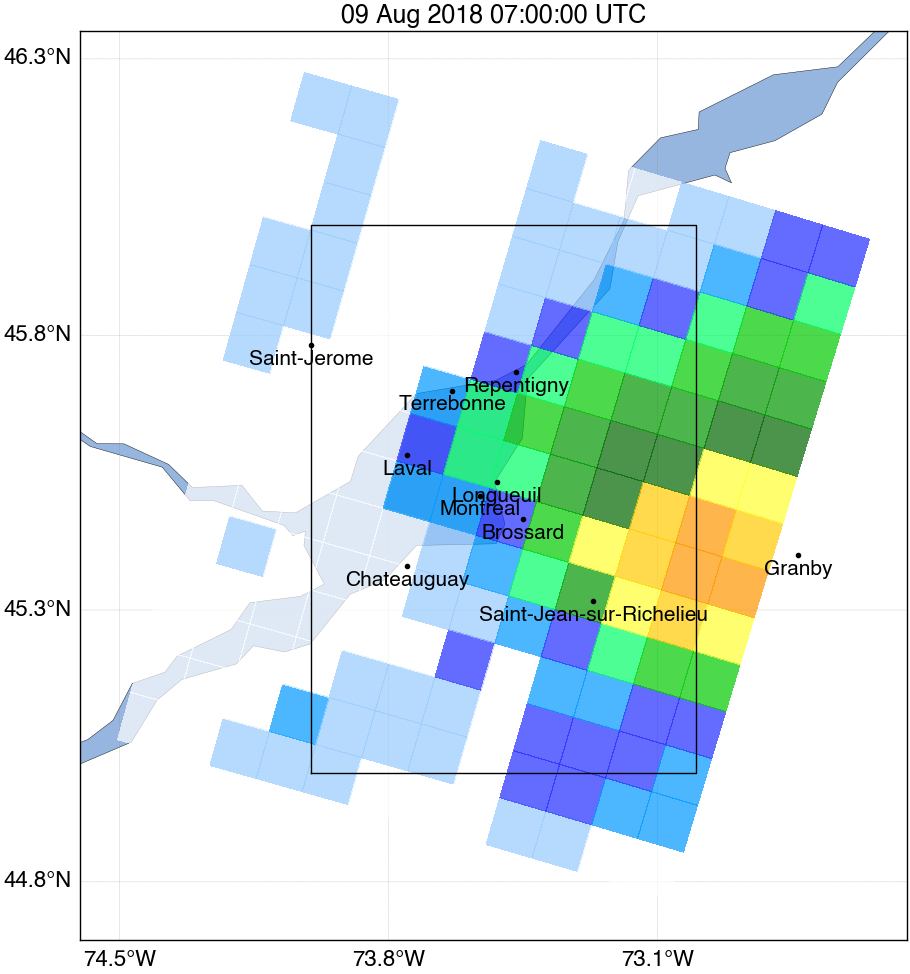
\includegraphics[height=0.9\linewidth]{figures/test-map-caspar-nrcan-hfe_2018080907.png}
		\caption{PNG produced using NRCan-HFE library based on NetCDF data (RDRS v2.1-1h) retrieved using \url{https://caspar-data.ca}}
		\label{fig:plot_example:caspar}
	\end{subfigure}
	\hspace*{0.02\textwidth}
	\begin{subfigure}[a]{0.1\textwidth}
		\centering
		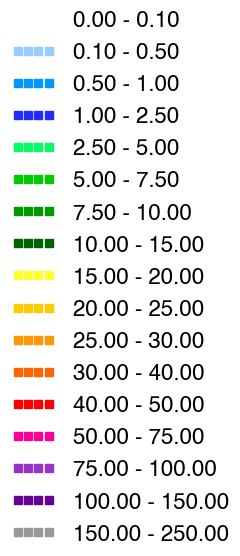
\includegraphics[width=\linewidth]{figures/test-map-caspar-nrcan-hfe_legend.png}
		\label{fig:plot_example:legend}
	\end{subfigure}
	\caption{RDPA (24h and 6h total precipitation) from Geomet and RDRS\_v2.1\_A\_PR0\_SFC (1h accumulations) from CaSPAr for data available for Aug 9, 2018. (a) RDPA-24h is accumulated precipitation for noon Aug 8, 2018 (UTC) until noon Aug 9, 2018 (UTC) \jm{(Vincent, RDPA-24h is period ending, right?)}, (b) RDPA-6h is accumulated precipitation for midnight Aug 9, 2018 (UTC) until 6am Aug 9, 2018 (UTC) \jm{(Vincent, RDPA-6h is period ending, right?)} while (c) RDRS-v2.1 is precipitation between Aug 9, 2018 6:00 am and 7:00 am (UTC) \jm{(Vincent, RDRS is period ending, right?)}. The same bounding box around Montreal has been requested from the three products. The panel in Fig.~\ref{fig:plot_example:api-weather:24h} is the same as panel in Fig.~\ref{fig:plot_example:api-weather}. The legend is the same for all plots.}
	\label{fig:plot_example_geomet-nrcan-hfe_vs_caspar-nrcan-hfe}
\end{figure}
\clearpage 

\section{Time sheet}

Listed hours spend per day with a brief description of activities are provided in Table~\ref{tab:hours}.
\begin{table}[h]
	\begin{tabular}{L{2cm}R{1cm}L{11.5cm}}
		\hline
		\textbf{Date} & \textbf{Hours} & \textbf{Description}\\
		\hline
		Aug 25, 2022 & 4 & Kick-off meeting; collecting resources; discussion GeoMet requests; documentation \\
		Aug 26, 2022 & 3 & discussion GeoMet requests; documentation \\
		Aug 27, 2022 & 12 & coding Geomet functions (a1, b1) and function to plot data (cx); documentation \\		
		Aug 28, 2022 & 12 & coding CaSPAr functions (a2, b2); refactor Geomet functions (a1, b1) and plotting (cx) for consistency; documentation \\	  
		\hline
		Sum & 31 & of 144 hrs in agreement\\
		\hline\hline
	\end{tabular}
	\caption{Project time sheet for Juliane Mai}
	\label{tab:hours}
\end{table}

\end{document}



